\documentclass{article}
\usepackage{graphicx}
\usepackage{amsmath,amssymb,mathrsfs,latexsym}
\usepackage[english]{babel}
\usepackage[T1]{fontenc}
\usepackage{makeidx}
\usepackage{algorithm}
\usepackage[noend]{algpseudocode}
\usepackage{subcaption}
\usepackage{enumitem}
\begin{document}

\tableofcontents
\pagebreak
\section{Description and modeling}
The general context is about the modeling of the N-Green network. Starting from an overall description of the model, state specifications of each component so we set the foundation for what deserves special attention and critical parameters to make it a simulation


\subsection{Description}
In the description of optical ring we consider node's two types. The first one is \textbf{bridge} and the second is\textbf{ switches}.\\
Indeed, the bridges are simple nodes of the ring capable of being the source or recipient of a packet within the ring. All their operations are internal to the ring. Switches are special nodes that delimit the size of the ring; They are also used for interconnecting the second ring and also they are able to empty containers without being recipient or source.\\ 

About  distribution modes we  mention the mode \textbf{Unicast} and \textbf{Broadcast-and-Select} that attract our attention.\\  In Unicast mode, each source node sends packets for a specific destination. This means that each container contains information for an exact destination and the same for waiting. It's called one-to-one\\For the Broadcast-and-Select mode, each source node uses the same slot to address a recipient set, and when they receive packets, they make a copy and then extract what is intended. It's named  one-to-many. The constraints are posed by the type of traffic and the requirements on slot's padding.\\ 

On the ring there are two types of services: \textbf{premium} and \textbf{best effort}. The premium means the high priority of packets or critical limits on which the delay must be as minimal as possible while the best effort is to satisfy as soon as possible. Even if it's a best effort, it will also be necessary to minimize the routing time as much as possible.\\

For packet's insertion, we have also two mode to explore: \textbf{opportunistic} and \textbf{reservation}.\\ 
The opportunistic insertion means that when a slot is empty, a node can use it to transmit some packets; the node may decide not to use it if it considers that none of the packets currently being build is ready for transmission.\\
About reservation mode, a slot may be empty but reserved for another node, or another class of service.\\
When a node is allowed to insert data, and there are several packets ready for insertion, the node has to select which one to insert: this is \textbf{scheduling}. The scheduling is internal to each node.\\

As regards the reception  on ring, a node decides to receive packet when it's label with receiver number. First case, the node may receive the packet and free the corresponding slot by erasing the packet; this is typical for the unicast mode. The second case, the node get an copy of the packet to check which data is for him exactly. Only the source of packet can erase and release slot.\\


\subsection{Model of Ring}
In this section we present the framework of defining our work, some specifications, problem and the approach of our observations.
\subsubsection{Slotted time model}
In our model the time is discrete. The unit of time is one slot. Let's note \textbf{ST} this time. With each ST click, each node sees a container with a capacity\textbf{c}. During the ST, two basics operations are possible:  \textbf{Writing} and  \textbf{Reading}.\\
In reading, it is a matter of making a copy of the packets to extract  data; for writing, put the packet to be sent. The packet''s weight can be noted  as to{$w_{p}$}


\subsubsection{Problem and Constraint}
On this part we summarize the constraint that can be used for the ring observation.\\
Let's note \textbf{R} the set of request, \textbf{$R_{p}$} $\subset$ R the set of request premium and  \\ \textbf{$R_{b}$} $\subset$ R the set of best effort request\\


$\forall$ r $\in$ \textbf{R} ;  {$t_{r}$}={$t_{e}$}+{$\alpha_{i}$} and  if  r $\in$ {$R_{p}$} $\Rightarrow$ {$\alpha_{i}$} $\rightarrow$ 0\\

thus,   $\min$ ($\sum$ {$\alpha_{i}$})\\

For slot using, Let's note  \textbf{$q_{i}$} length of request; and \textbf{P} as packet\\
{$q_{i}$}=const with const=$\max$({$q_{i}$})\\


     $\min$ $\sum$( C- {$W_{p}$})\\
{$W_{p}$}=$\sum$({$q_{i}$}) and $\beta$ =$ \frac{W_{p}}{C} $  where  $\beta$  $\rightarrow$ 1\\
 	
 
\subsubsection{About nodes} 
On a node, to manage request's list for preparation of packets to be sent. Each request has a arrival time  \textbf{$t_{a}$} which depend to period \textbf{p} of distribution on the ring.\\
 Whatever the type of request, it is necessary to be able to minimize the waiting time that's we note {$\alpha_{i}$} request for each node. Specially for premium request, the goal is to have no waiting time. Here It's important to explain how to create request on each node. On the ring we'll define period p for premium request creation on each node and quantity q. This implies that if we have request on time t on a node, the next request on the same node should be at t+p \\ 
Let's note  \textbf{MAX} maximum request production of the node 
\begin{algorithm}

\caption{creation of request}
\begin{algorithmic}
\State \textbf{Require:}  $start_{time}$; p
\State int $\delta$ =0;
\While{( $\neg$MAX)} 
\If{ $Current_{time}$ == $start_{time}$+$\delta$.p }
\State create request;
\State $\delta$++;
\EndIf
\EndWhile
\end{algorithmic}
\end{algorithm}  \\

For creating best effort request we'll use an uniform probability around the ring to add into all node this kind of request. All we need to use is the charge of ring.\\
Let's note $\delta$, $\sigma$ $\in$ [0;1] such as $\delta$ $\rightarrow$ 1 and  $\sigma$ $\rightarrow$ 0;
\begin{algorithm}
\caption{Best effort creation}
\begin{algorithmic}
\State \textbf{Require:}  $\sigma$, $\delta$
\If{ Uniform(0;1)$\geq$ $\delta$ \&  Uniform(0;1)$\geq$ $\sigma$ }
\State Create lots of Best effort
\Else
\State Create very little 
\EndIf
\end{algorithmic}
\end{algorithm}  

\subsubsection{Insertion} 
For emission problem we use the opportunistic strategy but the goal is to make a good use of resources. During ST, each node must use the container to put a packet as big as it's possible in order to avoid using too much resources than it's necessary. This is to avoid waste of resources and leave the charge of the ring very low. This seems to be somewhat in contradiction with the fact of minimizing the wait times of packets especially those of the service "premium"; But to restore the equilibrium, we will put a mechanism of right of access in emission on the containers in such a way that certain containers can be used only for priority packets. This is a good alternative to improve the time wasting by idea of filling the containers to be full at maximum. Another criteria we can add is to define an maximum waiting time which after this, the packets that we want to be full before sending must be sent even if it's not. This time can be noted \textbf{ {$\alpha_{max}$}}.

\begin{algorithm}
\caption{Packet's insertion}
\begin{algorithmic}
\State \textbf{Require:}  $\alpha_{max}$; $\beta$ $\in$ [0;1]
\If{$Creation_{time}$ -- $Current_{time}$ == $\alpha_{max}$ $\mid$  $\mid$ $ \frac{W_{p}}{C} $ $\geq$ $\beta$ }
\State send packet
\Else
\State wait for packing 
\EndIf
\end{algorithmic}
\end{algorithm}  
\newpage
\subsubsection{Latency}
Here we define latency as the difference between the time a request was received and the time it should be received if it was sending since the moment it was created. Indeed we can get a deterministic estimate of the time separating the path of a request between source and its destination noted as "best case". So the latency is mainly due to {$\alpha_{i}$}. Let's note latency as  \textbf{l}, the estimation sending time as  \textbf{ {$t_{e}$} } and the reel time of receive as { {$t_{r}$} } .\\

Two major problems stand out: minimizing {$\alpha_{i}$} and maximizing containers for message transport.
\subsection{Presentation of Model 1}

This part concerns the general problem that we study without any specification of the type of request that the node must send. This means that all is Best effort.\\
Let's note R=\{ $r_{1}$, $r_{2}$, $r_{3}$,......,$r_{i}$  \}, the list which can be request or best effort on this model.\\
\begin{algorithm}
\caption{Model 1}
\begin{algorithmic}
\State \textbf{Require:} R
\State $\forall$ r $\in$ R try removing from R to the sending packet's;
\State call \textbf{ Packet's insertion}
\end{algorithmic}
\end{algorithm}

\begin{figure}[h!]
  \begin{subfigure}[b]{0.9\textwidth}
    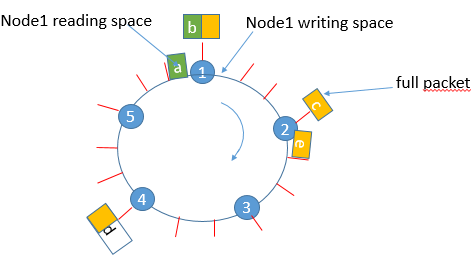
\includegraphics[width=\textwidth]{etape1.PNG}
    \caption{Picture 1}
    \label{fig:1}
  \end{subfigure}
  %
  \begin{subfigure}[b]{0.5\textwidth}
    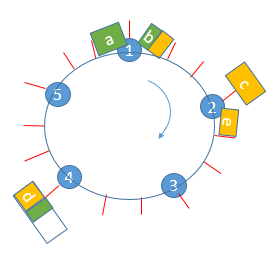
\includegraphics[width=\textwidth]{etape2.PNG}
    \caption{Picture 2}
    \label{fig:2}
  \end{subfigure}
%
  \begin{subfigure}[b]{0.5\textwidth}
    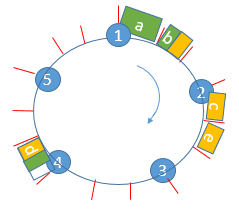
\includegraphics[width=\textwidth]{etape3.PNG}
    \caption{Picture 3}
    \label{fig:3}
  \end{subfigure}
\caption{Basic model1 view}
\end{figure}

\newpage
Figure 1: presents the model that we describe above and show how is the ring.
\begin{enumerate}[label=$\bullet$]
\item On Picture 1 the nodes 1,2 and 4 have respectively packets b, c and d on emission. Noticed that each node can read on left and read on right. So node 1 can read the packet a and puts its packet b on right.   
\item On picture 2 we can see the result of what is done during ST. Node 1 writes  on the slot at right and read on left. Node 2 can't write on the slot because the slot is used by packets e sending by another node. Node 4 doesn't write because the packet d isn't full enough for sending.
\item On picture 3, the next ST show that node 2 sends his packet by founding empty container and node 4 sends it too because packets d is full enough and ready to be sent .
\end{enumerate}

\subsection{Presentation of Model 2}
According to this model, node distinguishes the difference between request and best effort. So, for the node we model two packet's list: the first for requests and second for best effort. For sending, main solution is to empty the priority list before trying sending best effort. The goal for this model is to observe and compare with model 1 the gain for request versus loss for best effort.\\
Let's note $LP_{r}$ the list of packets for request sending; $LP_{b}$ the list of packets best effort.

\begin{algorithm}
\caption{Model 2 for priority }
\begin{algorithmic}
\State \textbf{Require:}  $LP_{r}$, $LP_{b}$
\While{($LP_{r}$ ! $\phi$)} 
\State call \textbf{ Packet's insertion} for $LP_{r}$
\EndWhile
\State call \textbf{ Packet's insertion} for $LP_{b}$
\end{algorithmic}
\end{algorithm}
\newpage
\begin{figure}
  \begin{subfigure}[b]{0.3\textwidth}
    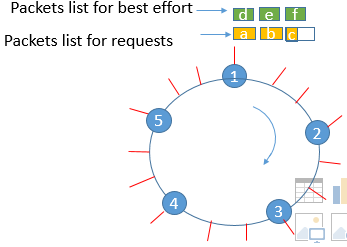
\includegraphics[width=\textwidth]{model21.PNG}
    \caption{Picture 1}
    \label{fig:1}
  \end{subfigure}
  %
  \begin{subfigure}[b]{0.3\textwidth}
    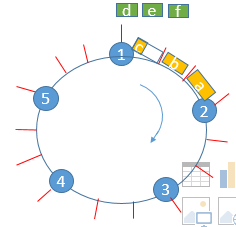
\includegraphics[width=\textwidth]{model22.PNG}
    \caption{Picture 2}
    \label{fig:2}
  \end{subfigure}
%
  \begin{subfigure}[b]{0.3\textwidth}
    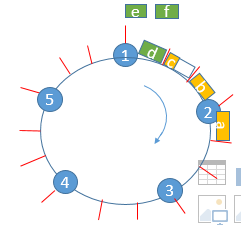
\includegraphics[width=\textwidth]{model23.PNG}
    \caption{Picture 3}
    \label{fig:3}
  \end{subfigure}
\caption{ model2 view}
\end{figure}

Figure 2: presents the sample model2 operation.
\begin{enumerate}[label=$\bullet$]
\item On Picture 1 the nodes 1 has two packets lists on emission. Request list contains a, b, c while best effort contains d, e, f.    
\item On picture 2 we can see the result of what is done after three ST. Node 1 sends all its priority packets before best effort. Noticed even if the packets c isn't full enough it was sent before best effort.
\item On picture 3, the next ST show that node 1 sends it's first best effort after having it's priority packet list empty.
\end{enumerate}


\subsection{Presentation of Model 3}
This model contains what we want improve after seeing mode 1 and 2. At first, get very fast as possible for priority packets like on model2; Avoid waste in the use of slot like model2, and improve waiting time for best effort and get it like in model1.\\
So, let's note\\
 $v_{r}$ $\subset$ $LP_{r}$ $\backslash$ $v_{r}$=\{ request \} and $v_{b}$ $\subset$ $LP_{r}$ $\backslash$ $v_{b}$=\{ request \} $\bigcup $ \{ best effort \} ; 
|$v_{r}$|=$\max$(|$v_{ri}$|) $\backslash$ $v_{ri}$  $\subset$ $LP_{r}$ ) and |$v_{b}$|=|$LP_{r}$|--|$v_{r}$|
For sending, algorithm is the same with model2; but we change best effort  insertion.


\begin{algorithm}
\caption{Best effort insertion}
\begin{algorithmic}
\State \textbf{Require:} b: best effort; $v_{r}$.Length; $v_{b}$.Length
\State find=false;
\While{$\neg$find} 
\If{|b| $\geq$ $v_{b}$.Length}
\State check place in the next $v_{r}$;
\EndIf
\EndWhile
\If{find}
\State put b in $v_{r}$ where place was found;
\Else
\State make insertion on $LP_{b}$;
\EndIf
\end{algorithmic}
\end{algorithm}
\newpage
\begin{figure}
  \begin{subfigure}[b]{0.3\textwidth}
    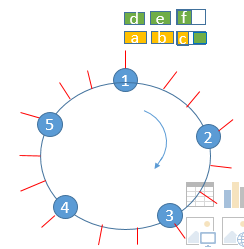
\includegraphics[width=\textwidth]{model31.PNG}
    \caption{Picture 1}
    \label{fig:1}
  \end{subfigure}
  %
  \begin{subfigure}[b]{0.3\textwidth}
    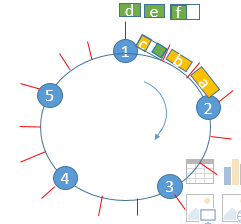
\includegraphics[width=\textwidth]{model32.PNG}
    \caption{Picture 2}
    \label{fig:2}
  \end{subfigure}
\caption{ model3 view}
\end{figure}


Figure 4: shows amelioration  we think for model3 by using the same picture as model2.
\begin{enumerate}[label=$\bullet$]
\item On Picture 1 the nodes 1 has two packets lists on emission. It's important to notice that the packets c which is not full is used by best effort. In this, the best effort what we put in is the head of packet d. d is looks full again because we put the e in it and f in queue of e. That's why f looks less full of best effort. 
\item On picture 2 we can see the result of what is done after three ST. 
\end{enumerate}

	 
\subsection{Model for  interconnection between two ring}
The second part of our work is about ring's interconnection. The problem that we have to solve is about lost of synchronization. When packets need to change node, difference between the slot's time click on the rings. we must point out our attention on the   \textbf{switch} node.\\
The node switch can erase container if it gets packets for another rings. So it means that he is a new 
transmitter of the packets. It's now important to think about how to use the container on the switch nodes. We can do it by using more ways.\\
\subsubsection{Priority to external packets}
In this case, it is considered that  on the switch node, priority will be given to the packets coming from an external node.The purpose of this is to minimize the additional waiting time for the packets on the waiting line of switch node. This could have very good results especially if inter-ring communications are even more numerous.\\

\subsubsection{Priority to internal packets}
In this case, it is considered that all priority is given to the packets inside the same ring. This results can be used when there isn't more packets between two rings. \\

\subsubsection{Mixed Priority}
With this model, we combine the two previous. So it's we can define an probabilistic aspect which can define when we get priority for internal packets or not.\\
 For sample, let's define  \textbf{$\Delta$} $\in$ [0;1]; \\

\begin{algorithm}
\caption{choose priority}
\begin{algorithmic}
\State \textbf{Require:} $\Delta$ $\in$ [0;1]
\If{$\Delta$ < 0.5}
\State return Priority to internal packets
\Else
\State return Priority to external packets
\EndIf
\end{algorithmic}
\end{algorithm}  


\subsubsection{Observations}
In this part we show the main problem we explain in interconnection case and describe what we exactly do.\\
\begin{figure*}[h!]
\begin{center}
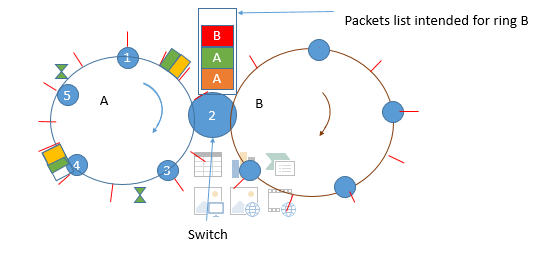
\includegraphics[scale=0.8]{inter1.PNG}
\caption{Rings interconnection}
\end{center}
\end{figure*}

Figure 3: presents the model that we describe above and show what happen on switch node. Here we show on node 2 a sample of move on this node. Node 2 packet's waiting list. On the list we have as much packets coming from ring A to B as packets which are introduced for ring B.
\clearpage
\begin{figure}
  \begin{subfigure}[b]{0.6\textwidth}
    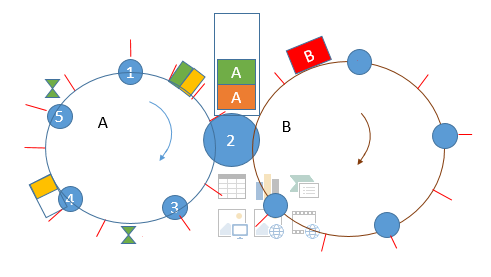
\includegraphics[width=\textwidth]{inter2.PNG}
    \caption{Internal priority}
    \label{fig:1}
  \end{subfigure}
  %
  \begin{subfigure}[b]{0.6\textwidth}
    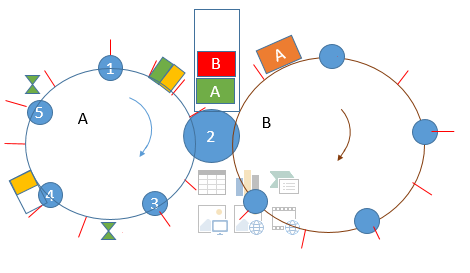
\includegraphics[width=\textwidth]{inter3.PNG}
    \caption{external priority}
    \label{fig:2}
  \end{subfigure}
\caption{Priority choice}
\end{figure}
Figure4: show us the different possibility for the switch to manage the list.\\
In (a) packets which source is the ring B is chosen to be put on the slot but in (b), the stranger pass at first.\\

Let's consider {$T_{A}$} , {$T_{B}$} the time that need packets turn around  ring A and B respectively. And also consider {$T_{R}$ as real time for packets transmission.\\
The goal to obtain:   {$T_{R}$  $\leq$ {$T_{A}$} + {$T_{B}$}.



\end{document}